%!TEX root = ../../Main.tex
\graphicspath{{Chapters/Identifikation_af_open_loop_system/}}
%-------------------------------------------------------------------------------

\section{Identifikation af open-loop system}

Efter vi har besluttet os for hvilket system vi ønskede at designe, og hvilke dele systemet skal bestå af, er det næste skridt at indsamle data fra vores motor via den indlagte encoder. Det gør vi ved at sende et step input ind på motoren. Vi aflæser to outputs, både det direkte output fra encoderen, som er rotationen i grader, samt den afledte som er hastigheden i grader. Opstillingen af denne måling i Simulink kan ses på \autoref{fig:Simulink_opstilling_af_maaling}. Disse målinger gentog vi mange gange, for at få de bedst mulige målinger. Grunden til at vi ønsker de bedste mulige målinger er, så vi kan lave den bedst mulige repræsentation af vores system, så det system vi beregner på, er så tæt på det faktiske system som overhovedet muligt.
  
\begin{figure}[H]
	\centering
	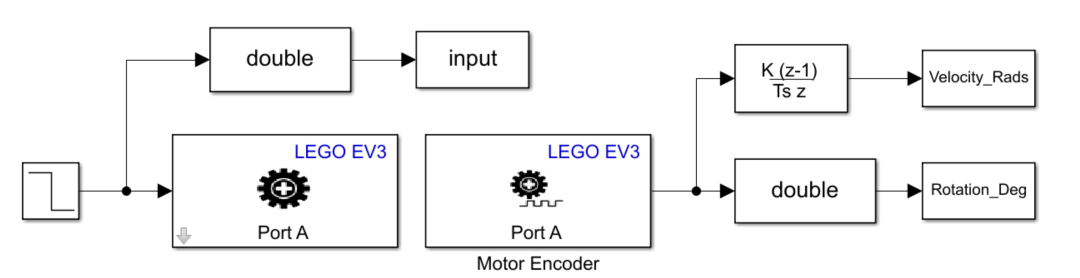
\includegraphics[width = 400pt]{Img/Simulink_opstilling_af_maaling.png}
	\caption{Simulink opstilling af måling}
	\label{fig:Simulink_opstilling_af_maaling}
\end{figure}

Grafen på \autoref{fig:Motor_deg_graf} repræsenterer motorens rotation i grader. Grafen på \autoref{fig:Motor_velocity_graf} repræsenterer den afledte af positionen i grader, altså hastigheden i grader. Som man kan se på \autoref{fig:Motor_velocity_graf} opfører den afledte sig som et første ordens system, dog med et lille udfald i accelerationen, men da den er så lille vælger vi at se bort fra denne. Da vores afledte opfører sig som et første ordens system må det betyde at vores system er et 2. ordens system. 

\begin{figure}[H]
	\centering
	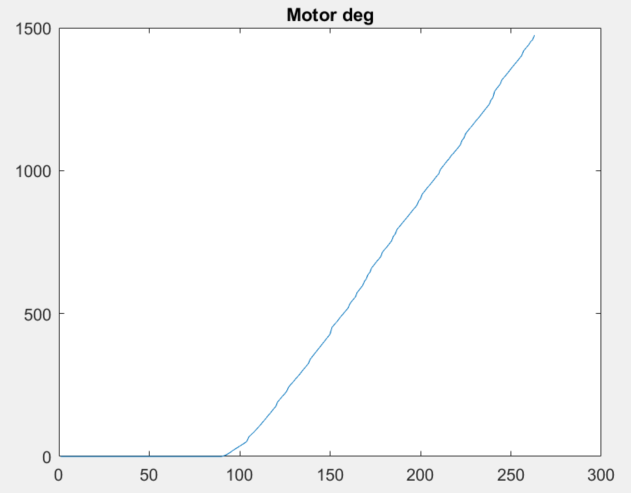
\includegraphics[width = 300pt]{Img/Motor_deg_graf.png}
	\caption{Måling af motor vinkel i grader}
	\label{fig:Motor_deg_graf}
\end{figure}

\begin{figure}[H]
	\centering
	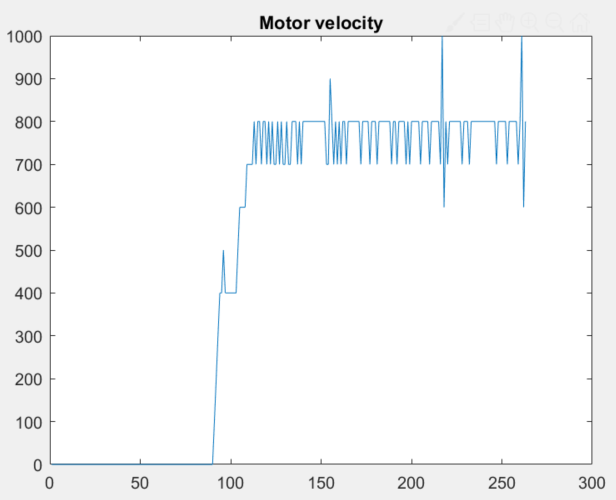
\includegraphics[width = 300pt]{Img/Motor_velocity_graf.png}
	\caption{Måling af motorens hastighed i grader}
	\label{fig:Motor_velocity_graf}
\end{figure}

Vi besluttede os for at gå videre med disse målinger, og benyttede os af "tfest" funktionen i matlab til, ud fra vores data, at estimere en 2. ordens transfer funktionen. 
\begin{equation}
\frac{74.34}{s^2+8.028s+0.1365}
\end{equation}


Vi ønsker at opstille vores system på state space form, da det gør det mulig at evaluere systemet ved hjælp af matrix algebra. State space er specielt brugbart i systemer med flere input og flere outputs, i kontrast til klassisk kontrol metoder, så som PID-regulering, som bygger på komplekse lapace og fourier ligninger, som skal transformeres frem og tilbage mellem tids- og frekvensdomænet. 
En af de helt store fordele ved state space kontrol er dens anvendelighed til et bredt spekter af systemer, det kan både anvendes på linær og ikke linære, tidsafhængelige og tids uafhændelige, single-input single-output og multiple-input og multiple-output systemer.
State space bliver repræsenteret ved bare to ligninger. Første ligning, som ses på \autoref{eq:StateSpace_form1}, giver forholdet mellem systemets nuværende state og den afledte state. \autoref{eq:StateSpace_form2} viser at systemets output er afhængig af systemets nuværende state. På \autoref{fig:StateSpaceBlockDiagram} ses et state space block diagram. \begin{equation}
\dot{x} = A * x(t) + B * u(t)
\label{eq:StateSpace_form1}
\end{equation}
\begin{equation}
y = C * x(t) + D * u(t)
\label{eq:StateSpace_form2}
\end{equation}
\\
Hvor:\\
x er en vektor af alle state variabler\\
x' er en vektor af de afledte state variabler\\
A matrix er state matrixen  \\
B matrix er input matrixen \\
C matrix er output matrixen\\
D matrix er feedforward matrixen\\

\begin{figure}[H]
	\centering
	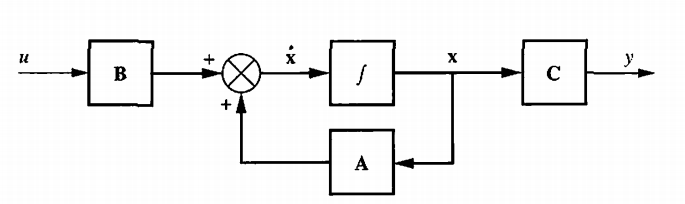
\includegraphics[width = 300pt]{Img/StateSpaceBlockDiagram.PNG}
	\caption{State space block diagram uden D}
	\label{fig:StateSpaceBlockDiagram}
\end{figure}



Derfor ønsker vi nu at få opstillet vores transfer funktion på state space form, det gør vi med matlab funktionen ”tf2ss”, som transformere vores transfer funktion til state space controllable canonical form. Denne state space repræsentation kan ses på \autoref{eq:StateSpace_AogB} og \autoref{eq:StateSpaceC}. Vores D matrice er lige 0, og derfor ikke med i vores state space repræsentation.

\begin{equation}
	\begin{bmatrix}
	\dot{x_1}   \\
	\dot{x_2}   \\
	\end{bmatrix}
	=
	\begin{bmatrix}
	0       &  1  \\
	-0.137      & -8.28 \\
	\end{bmatrix}
	*
	\begin{bmatrix}
	x_1   \\
	x_2   \\
	\end{bmatrix}
	+
	\begin{bmatrix}
	0   \\
	1   \\
	\end{bmatrix}
		*
	u
	\label{eq:StateSpace_AogB}
\end{equation}


\begin{equation}
	y
=
\begin{bmatrix}
74.340      &  0  \\
\end{bmatrix}
*
\begin{bmatrix}
x_1   \\
x_2   \\
\end{bmatrix}
\label{eq:StateSpaceC}
\end{equation}


Vi har ud fra vores målinger estimeret en transfer funktion, og sat den op på state space form, og er nu klar til pol placering, som vil blive forklaret i næste afsnit. 


\newpage